\section{效率的测量}
\def\effTot{\ensuremath{\epsilon_{\mathrm{tot}}}\xspace}
\def\effAcc{\ensuremath{\epsilon_{\mathrm{acc}}}\xspace}
\def\effReco{\ensuremath{\epsilon_{\mathrm{rec\&sel}}}\xspace}
\def\effID{\ensuremath{\epsilon_{\mathrm{MuonID}}}\xspace}
\def\effTrigger{\ensuremath{\epsilon_{\mathrm{Trigger}}}\xspace}
 
$\lhcb$上总的效率$\varepsilon_{tot}$由四部分组成:接受度效率$\effAcc$、重建选择效率$\effReco$、粒子鉴别效率$\effID$、触发效率$\effTrigger$,总的效率$\effTot$的计算公式如~\ref{eq:tot}所示:
效率主要是通过MC进行研究,$\pp$对撞直接产生的$\psitwos$介子和来自$b$强子衰变的$\psitwos$介子的效率有可能会有轻微的差别,我们对这二者分开进行计算。
\begin{equation}
  \effTot = \effAcc \times \effReco \times \effID \times \effTrigger,
\label{eq:tot}
\end{equation}

\subsection{接受度效率}
接受度效率的研究思路,如公式~\ref{eq:acceptance}所示:
\begin{equation}\label{eq:acceptance}
\effAcc \equiv \frac{\mbox{子区间 \textrm{($p_{\rm T}$,$y$)} 中$\psitwos$衰变而来的两个$\mu$都在$\lhcb$接受范围内的$\psitwos$}}{\mbox{子区间 \textrm{($p_{\rm T}$,$y$)} 中产生的$\psitwos$}}.
\end{equation}
公式的分子中要求两个$\mu$的极角(相对$z$轴的夹角)在$[10,400]\mrad$的范围内。
图~\ref{fig:EffAcc}给出了直接产生的$\psitwos$介子和来自$b$强子衰变的$\psitwos$介子的接受度效率分布。
%%%%%%%%%%%%%%%%%%%%%%%%%%%%%%%%%%%%%%%%%%%%%%%%%%%%%%%%%%%
\begin{figure}[!tbp]
\centering
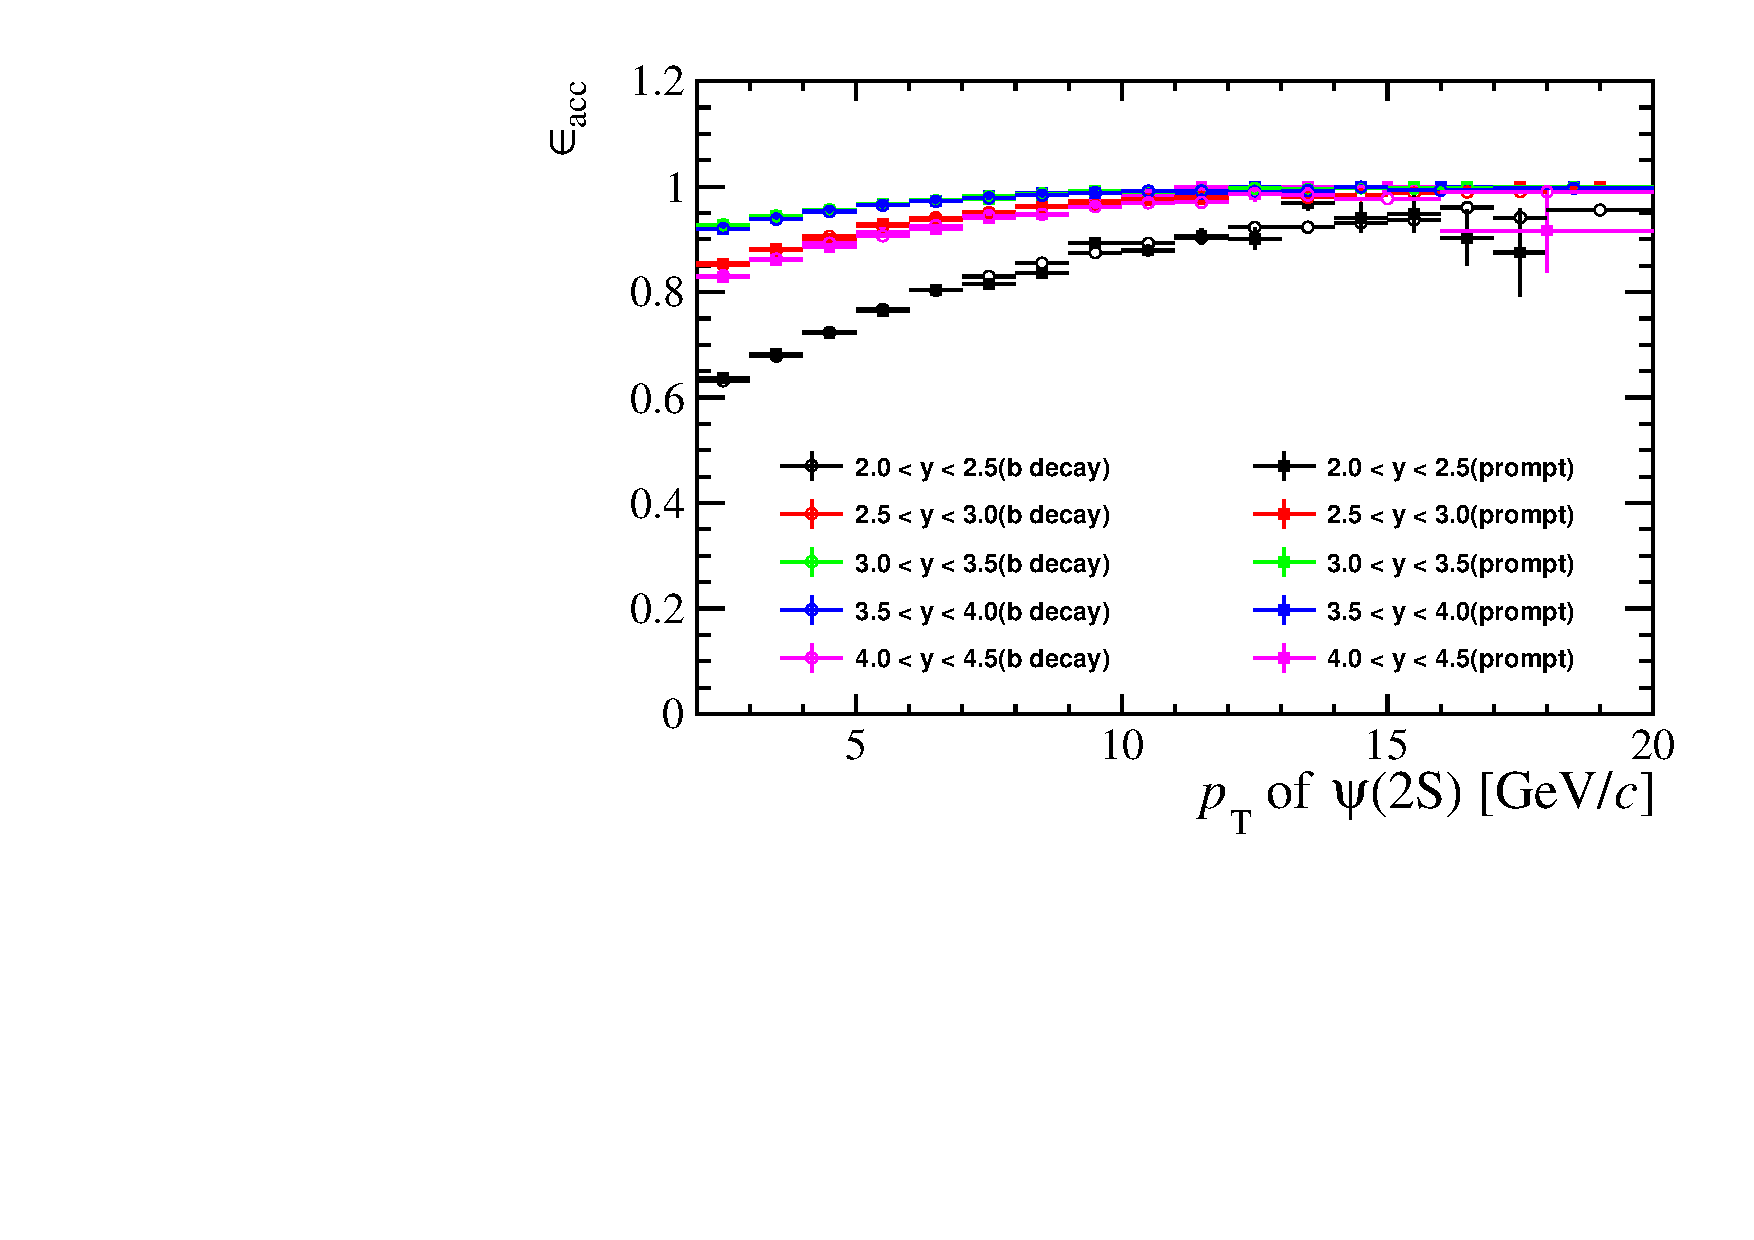
\includegraphics[width=0.9\textwidth]{chap3_eff_acc_compare}
\caption{以$\pt$、$y$为函数的接受度效率分布。}
\label{fig:EffAcc}
\end{figure}
%%%%%%%%%%%%%%%%%%%%%%%%%%%%%%%%%%%%%%%%%%%%%%%%%%%%%%%%%%


\subsection{重建选择效率}
重建选择效率计算公式如下所示:
\begin{equation}
  \effReco \equiv \frac{\mbox{子区间 \textrm{($p_{\rm T}$,$y$)} 中被探测且经过了重建选择但未加$PID_{\mu}$要求的$\psitwos$}}{\mbox{子区间 \textrm{($p_{\rm T}$,$y$)} 中$\psitwos$衰变而来的两个$\mu$子都在$\lhcb$接受范围内的$\psitwos$}}.
\end{equation}
重建选择效率包含了表~\ref{tab:selections}除了粒子鉴别之外其它所有涉及到径迹重建的效率。

研究表明MC得出的效率和真实数据中的效率有些差别,我们需要按照给定的效率修正表~\ref{fig:TrackEfficiencyCalib}来进行修正。
在每个($\pt$,$y$)的区间之内修正重建效率之前,我们先对MC事例多重数进行了修正,使其分布和数据保持一致,见图~\ref{fig:nspd}。因为多重数也会影响效率的计算。

%%%%%%%%%%%%%%%%%%%%%%%%%%%%%%%%%%%%%%%%%%%%%%%%%%%%%%%%%%%
\begin{figure}[!tbp]
\centering
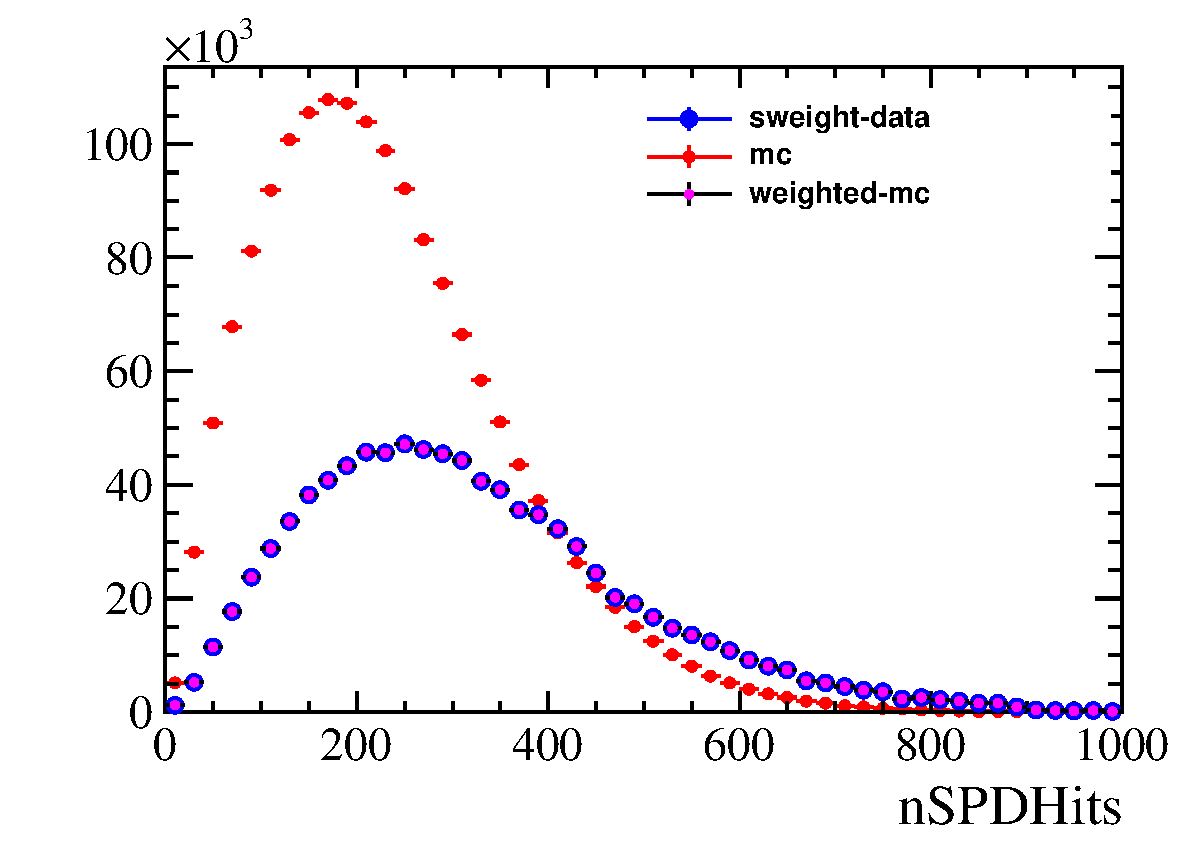
\includegraphics[width=0.9\textwidth]{chap3_reweight_nspd}
\caption{数据和MC中多重数的分布。}
\label{fig:nspd}
\end{figure}
%%%%%%%%%%%%%%%%%%%%%%%%%%%%%%%%%%%%%%%%%%%%%%%%%%%%%%%%%%
%%%%%%%%%%%%%%%%%%%%%%%%%%%%%%%%%%%%%%%%%%%%%%%%%%%%%%%%%%%
\begin{figure}[!tbp]
\centering
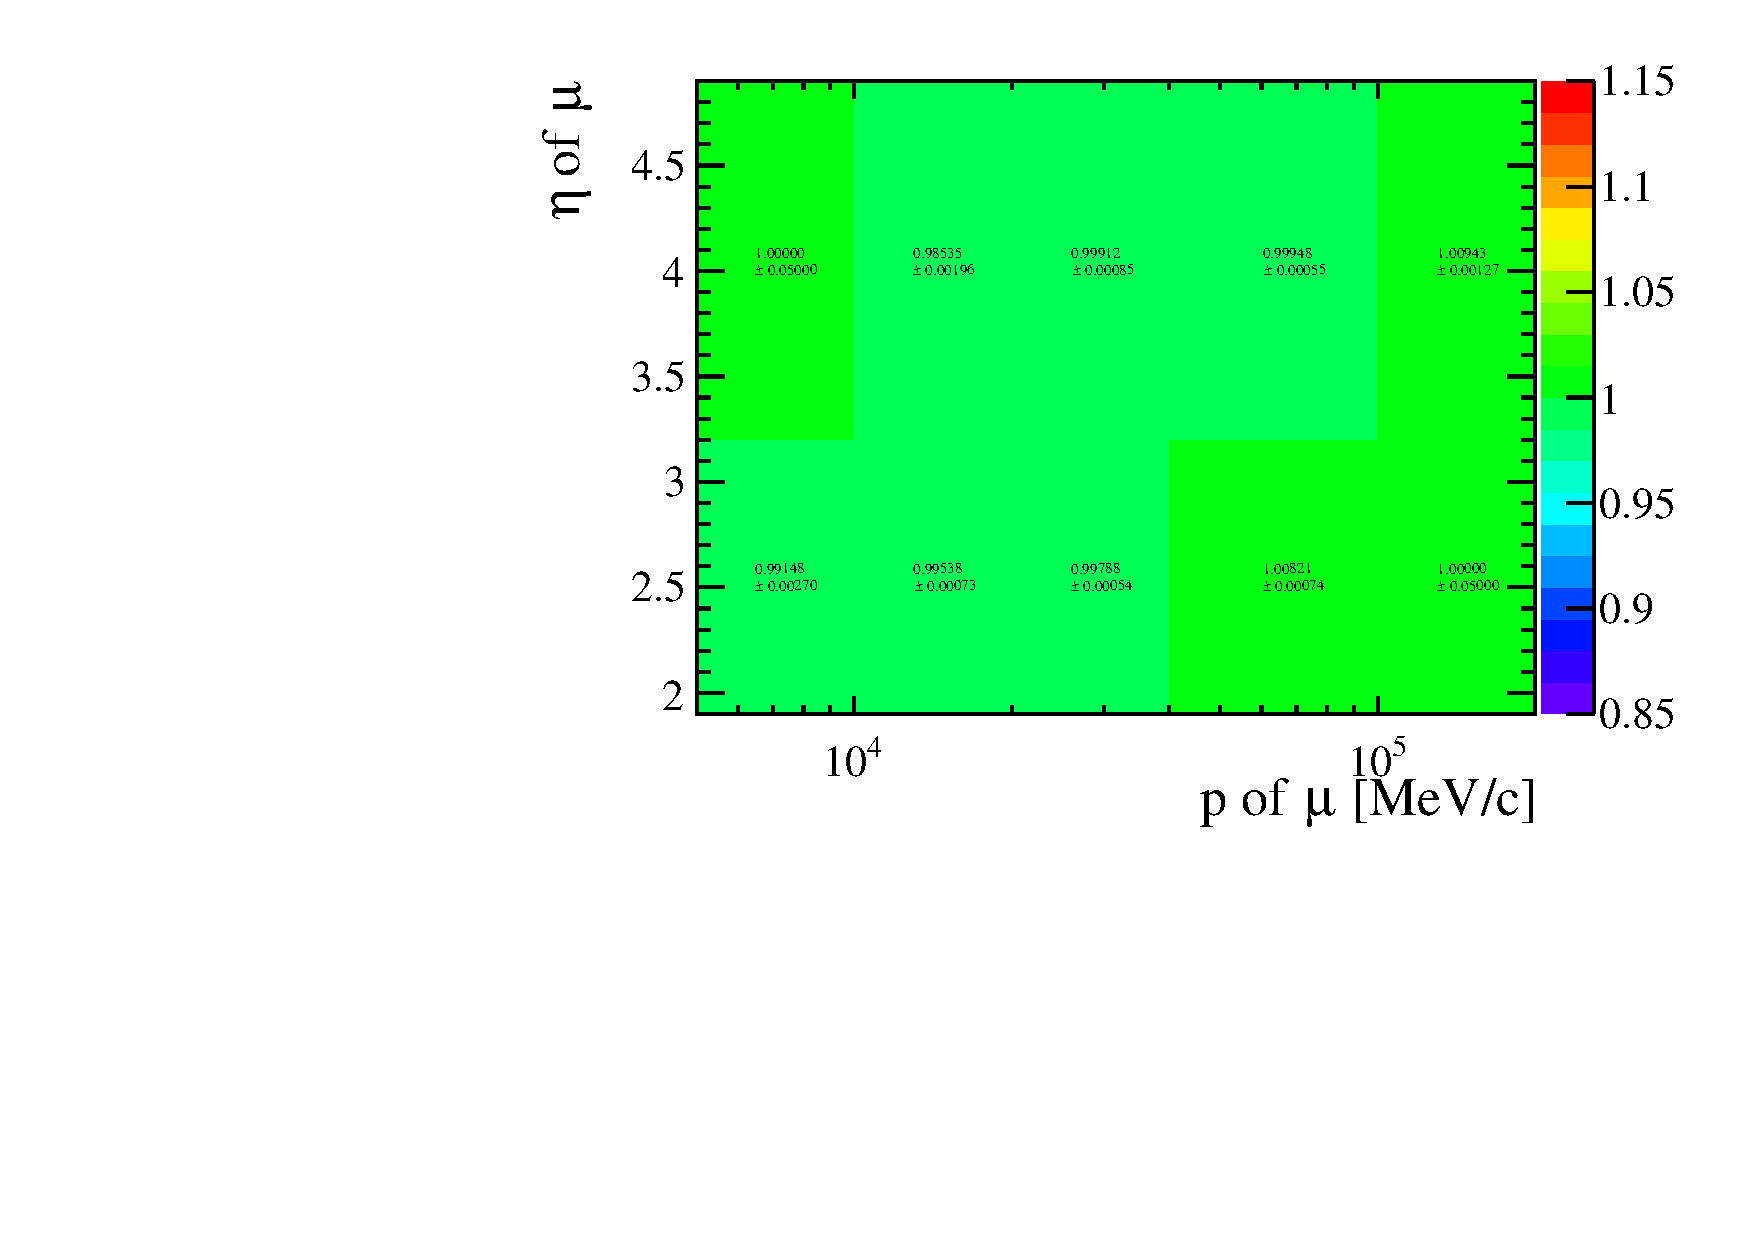
\includegraphics[width=0.9\textwidth]{chap3_Ratio_MCdata}
\caption{在每个$p_\mu$和$\eta_\mu$的区间之内,MC和数据的效率修正表。}
\label{fig:TrackEfficiencyCalib}
\end{figure}

对于每一个$\pt$,$y$ 区间,重建选择效率 $\effReco$的分布见图~\ref{fig:EffRec}, 
需要指出在研究重建选择效率的时候,对于$\pp$对撞直接产生的$\psitwos$ 介子和来自$b$强子衰变产生的$\psitwos$介子效率略有差异,原因主要有两个:一个是因为来自$b$强子的事例有较大的径迹重建数;另一个原因是来自$b$强子的事例有一个大约1.5 ps的有效寿命。
%%%%%%%%%%%%%%%%%%%%%%%%%%%%%%%%%%%%%%%%%%%%%%%%%%%%%%%%%%%
\begin{figure}[!tbp]
\centering
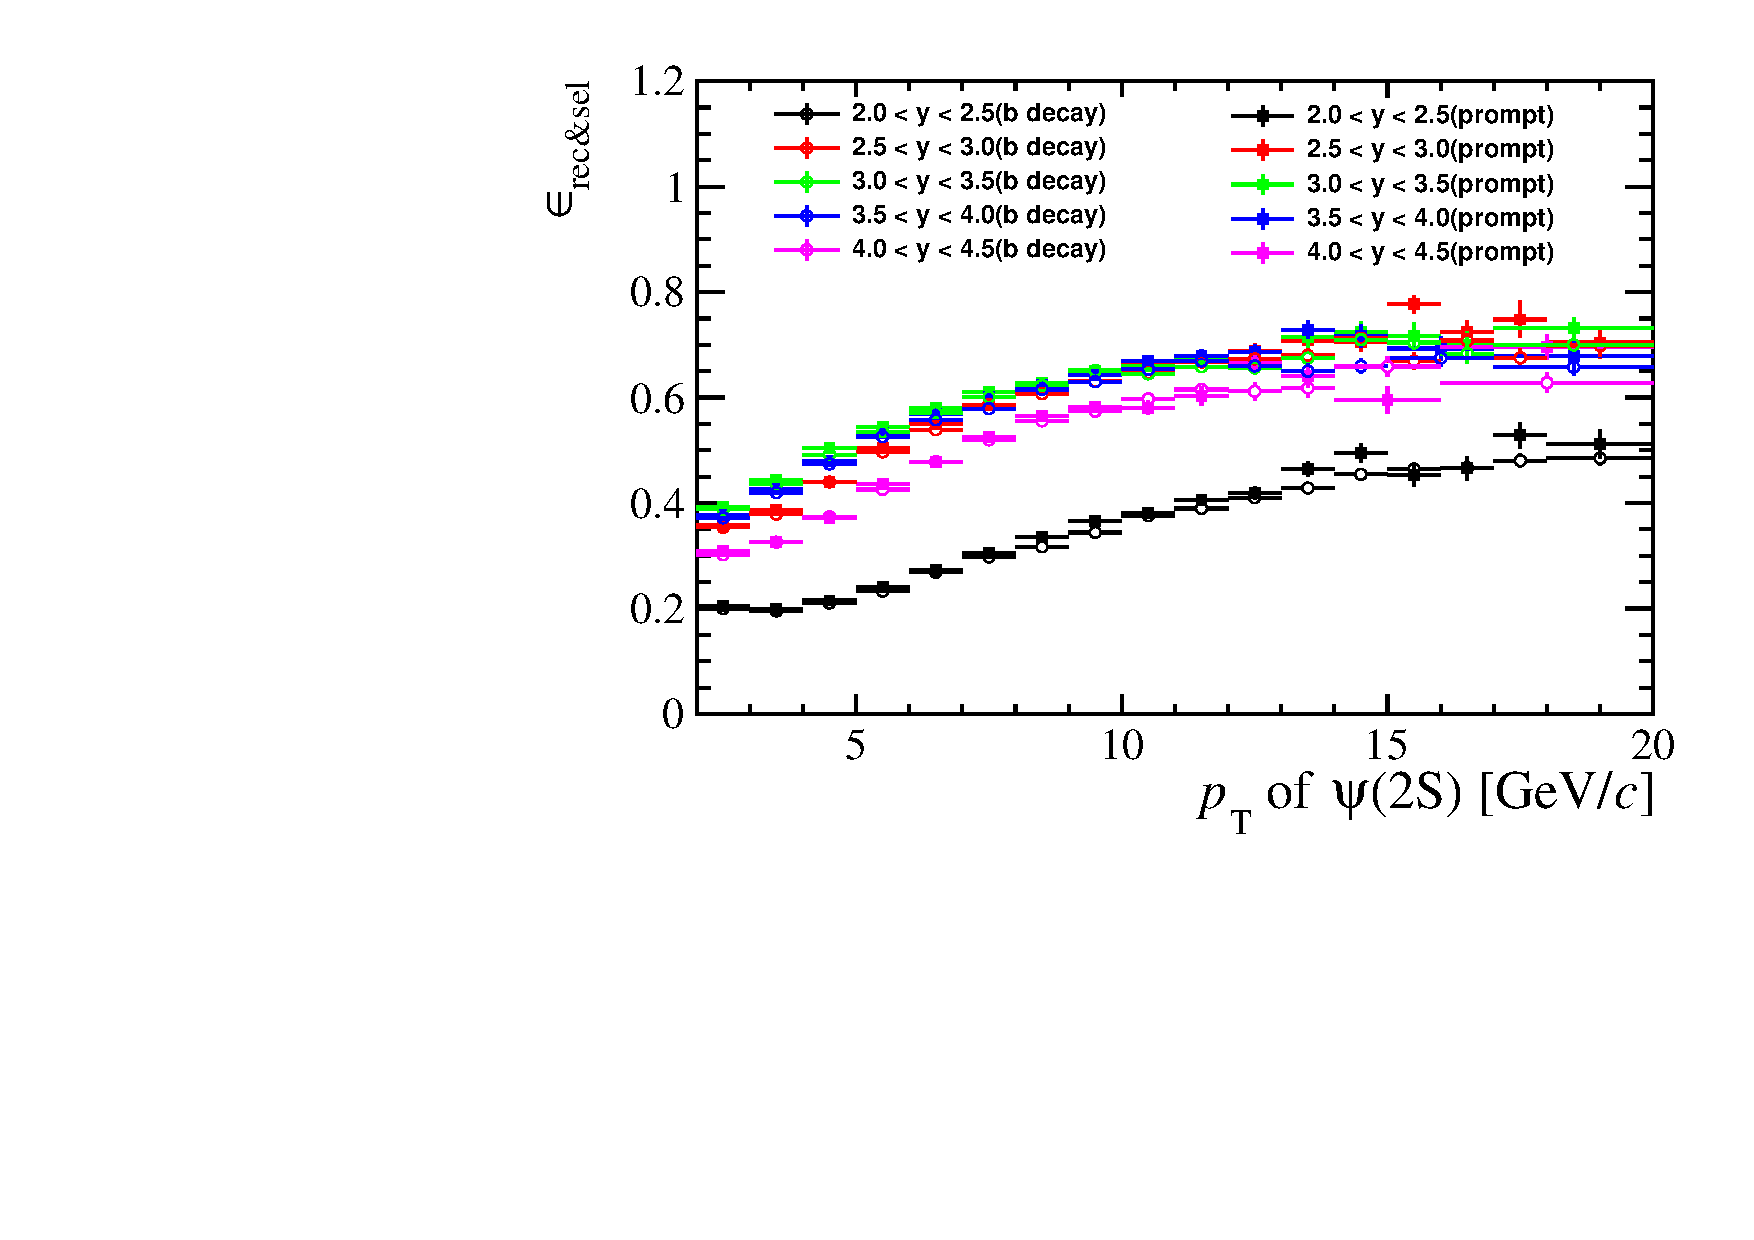
\includegraphics[width=0.9\textwidth]{chap3_eff_recsel_compare}
\caption{以$\pt$、$y$为函数的重建选择效率分布图。}
\label{fig:EffRec}
\end{figure}
%%%%%%%%%%%%%%%%%%%%%%%%%%%%%%%%%%%%%%%%%%%%%%%%%%%%%%%%%%

\subsection{$\mu$的粒子鉴别效率}
对于$\mu$的粒子鉴别效率的研究,研究思路如公式所示:
\begin{equation}
\effID \equiv \frac{\mbox{子区间 \textrm{($p_{\rm T}$,$y$)} 中被探测且经过了重建选择并加了$PID_{\mu}$要求的$\psitwos$}}{\mbox{子区间 \textrm{($p_{\rm T}$,$y$)} 中被探测且经过了重建选择但未加$PID_{\mu}$ 要求的$\psitwos$}}.
\end{equation}

实际计算的时候,我们依然采用MC样本计算,然后用控制样本来修正MC数据差异的方式。
PID calibration效率表是一个$p-\eta-nSPDhits$的三维表,这里用nSPD的击中数代表了径迹的多重数。
在每一个(\pt,$y$)的运动学区间内,我们根据此区间内每个事例的效率值进行平均得到该区间内的效率值。
而每个事例的效率是通过两个$\mu$的效率(依赖于各自的$(p,\eta,nSPDhits)$)的乘积来进行计算。
具体的计算公式如下:
\begin{equation}
\overline{\epsilon}(\pt,y)=\frac{\sum \epsilon_\mup(p_\mup,\eta_\mup,\mathrm{nSPDhits})\epsilon_\mun(p_\mun,\eta_\mun,\mathrm{nSPDhits})}{N_\mathrm{res\&sel}}.
\label{eq:muonid}
\end{equation}
其中 $\epsilon_\mup(p_\mup,\eta_\mup,\mathrm{nSPDhits})$ 和 $\epsilon_\mun(p_\mun,\eta_\mun,\mathrm{nSPDhits})$是来自于效率修正表修正之后的效率值。
每一个(\pt,$y$)的运动学区间内,$\mu$的粒子鉴别效率 \effID 展示在图~\ref{fig:EffID}内。

%%%%%%%%%%%%%%%%%%%%%%%%%%%%%%%%%%%%%%%%%%%%%%%%%%%%%%%%%%%
\begin{figure}[!tbp]
\centering
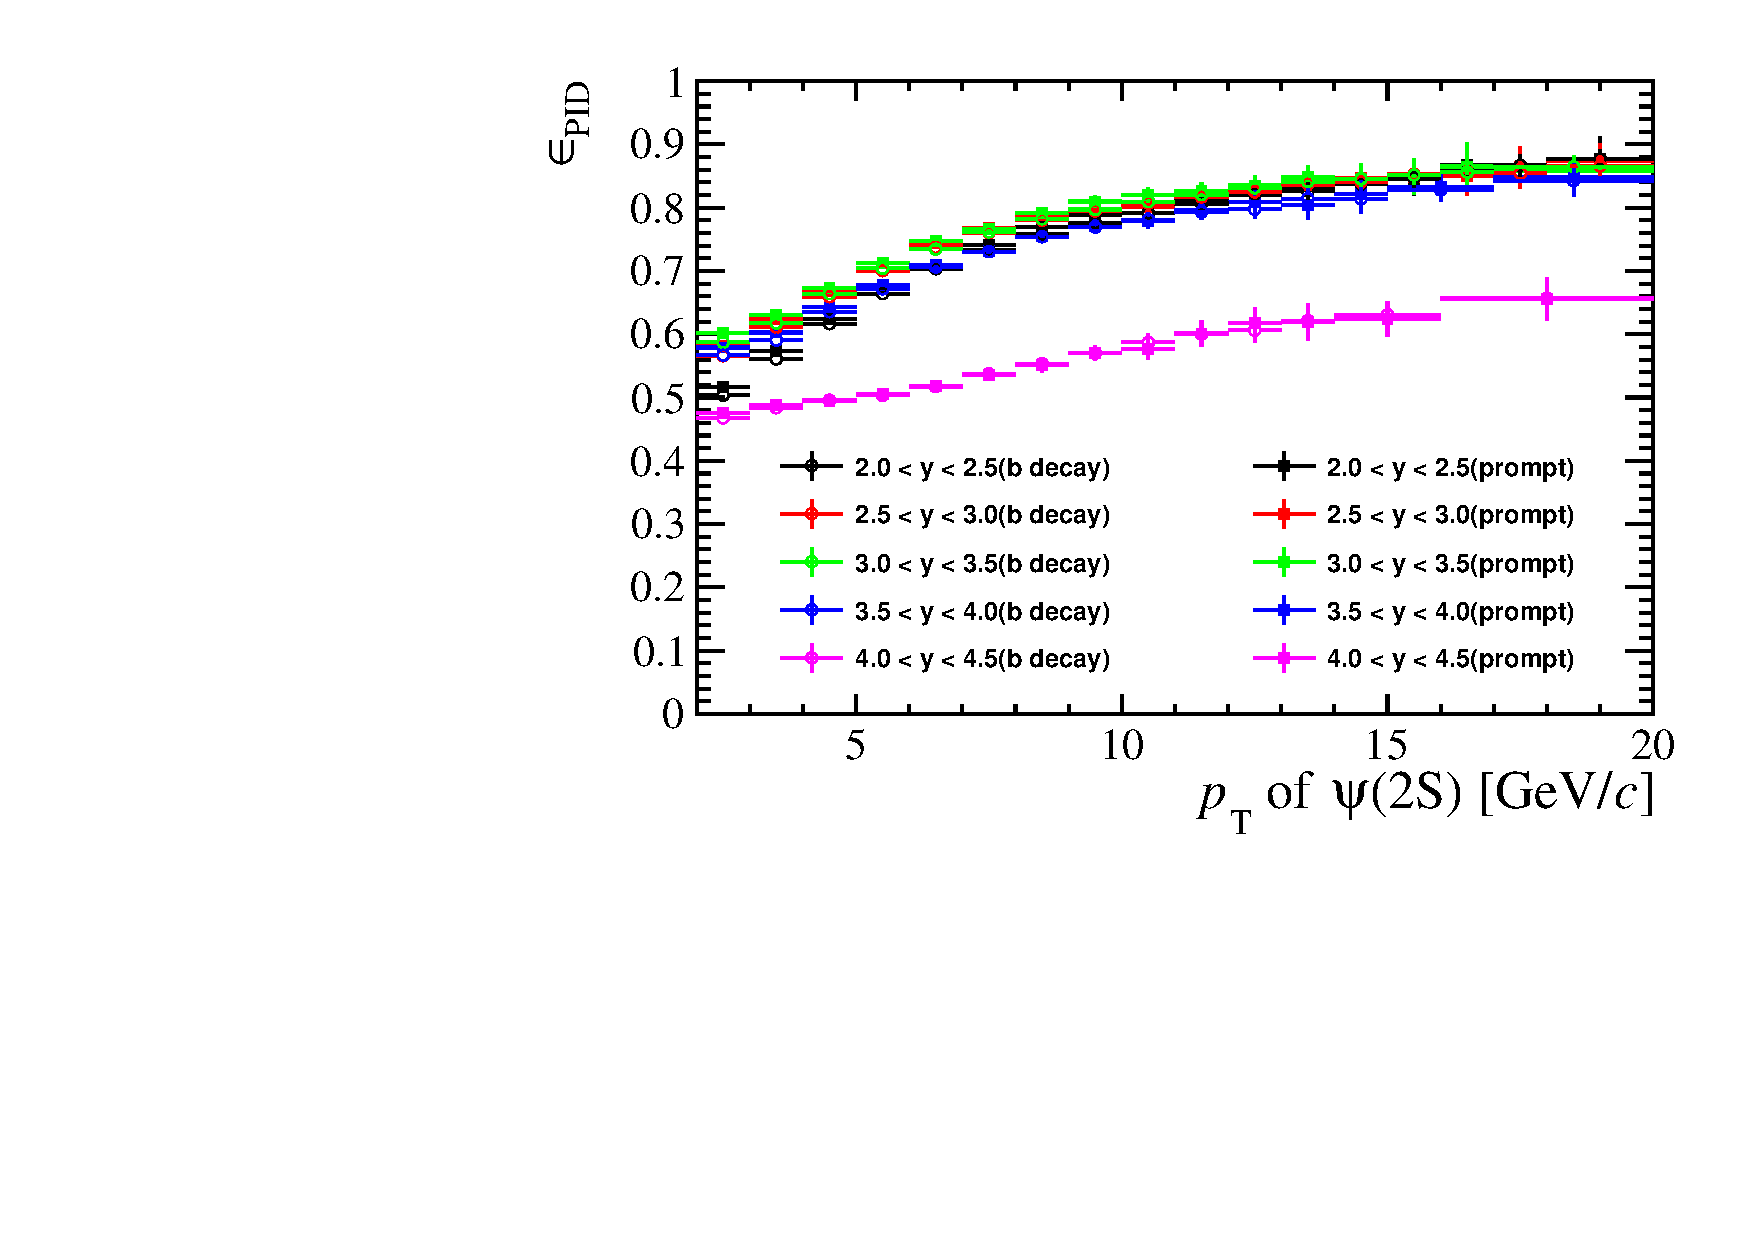
\includegraphics[width=0.9\textwidth]{chap3_eff_pid_compare}
\caption{以$\pt$、$y$为函数的$\mu$粒子鉴别效率分布。}
\label{fig:EffID}
\end{figure}
%%%%%%%%%%%%%%%%%%%%%%%%%%%%%%%%%%%%%%%%%%%%%%%%%%%%%%%%%%

\subsection{触发效率}

触发效率的计算公式下所示:
\begin{equation}
\effTrigger \equiv \frac{\mbox{加了分母中的选择条件且经过触发之后的$\psitwos$}}{\mbox{子区间 \textrm{($p_{\rm T}$,$y$)} 中被探测且经过了重建选择并加了$\mu$ 粒子鉴别要求的$\psitwos$}}
\end{equation}
在效率计算中,起主要贡献的仅仅是L0Dimuon和Hlt1DimuonHighMass这两部分,而对Hlt2DimuonPsi2STrubo这部分的效率几乎是100\%,因为离线选择条件比起Hlt2DimuonPsi2STrubo而言,加了更紧的条件。
每个($\pt$,$y$)区间内,触发效率$\effTrigger$的分布图如~\ref{fig:EffTrigger}所示。
%%%%%%%%%%%%%%%%%%%%%%%%%%%%%%%%%%%%%%%%%%%%%%%%%%%%%%%%%%%
\begin{figure}[!tbp]
\centering
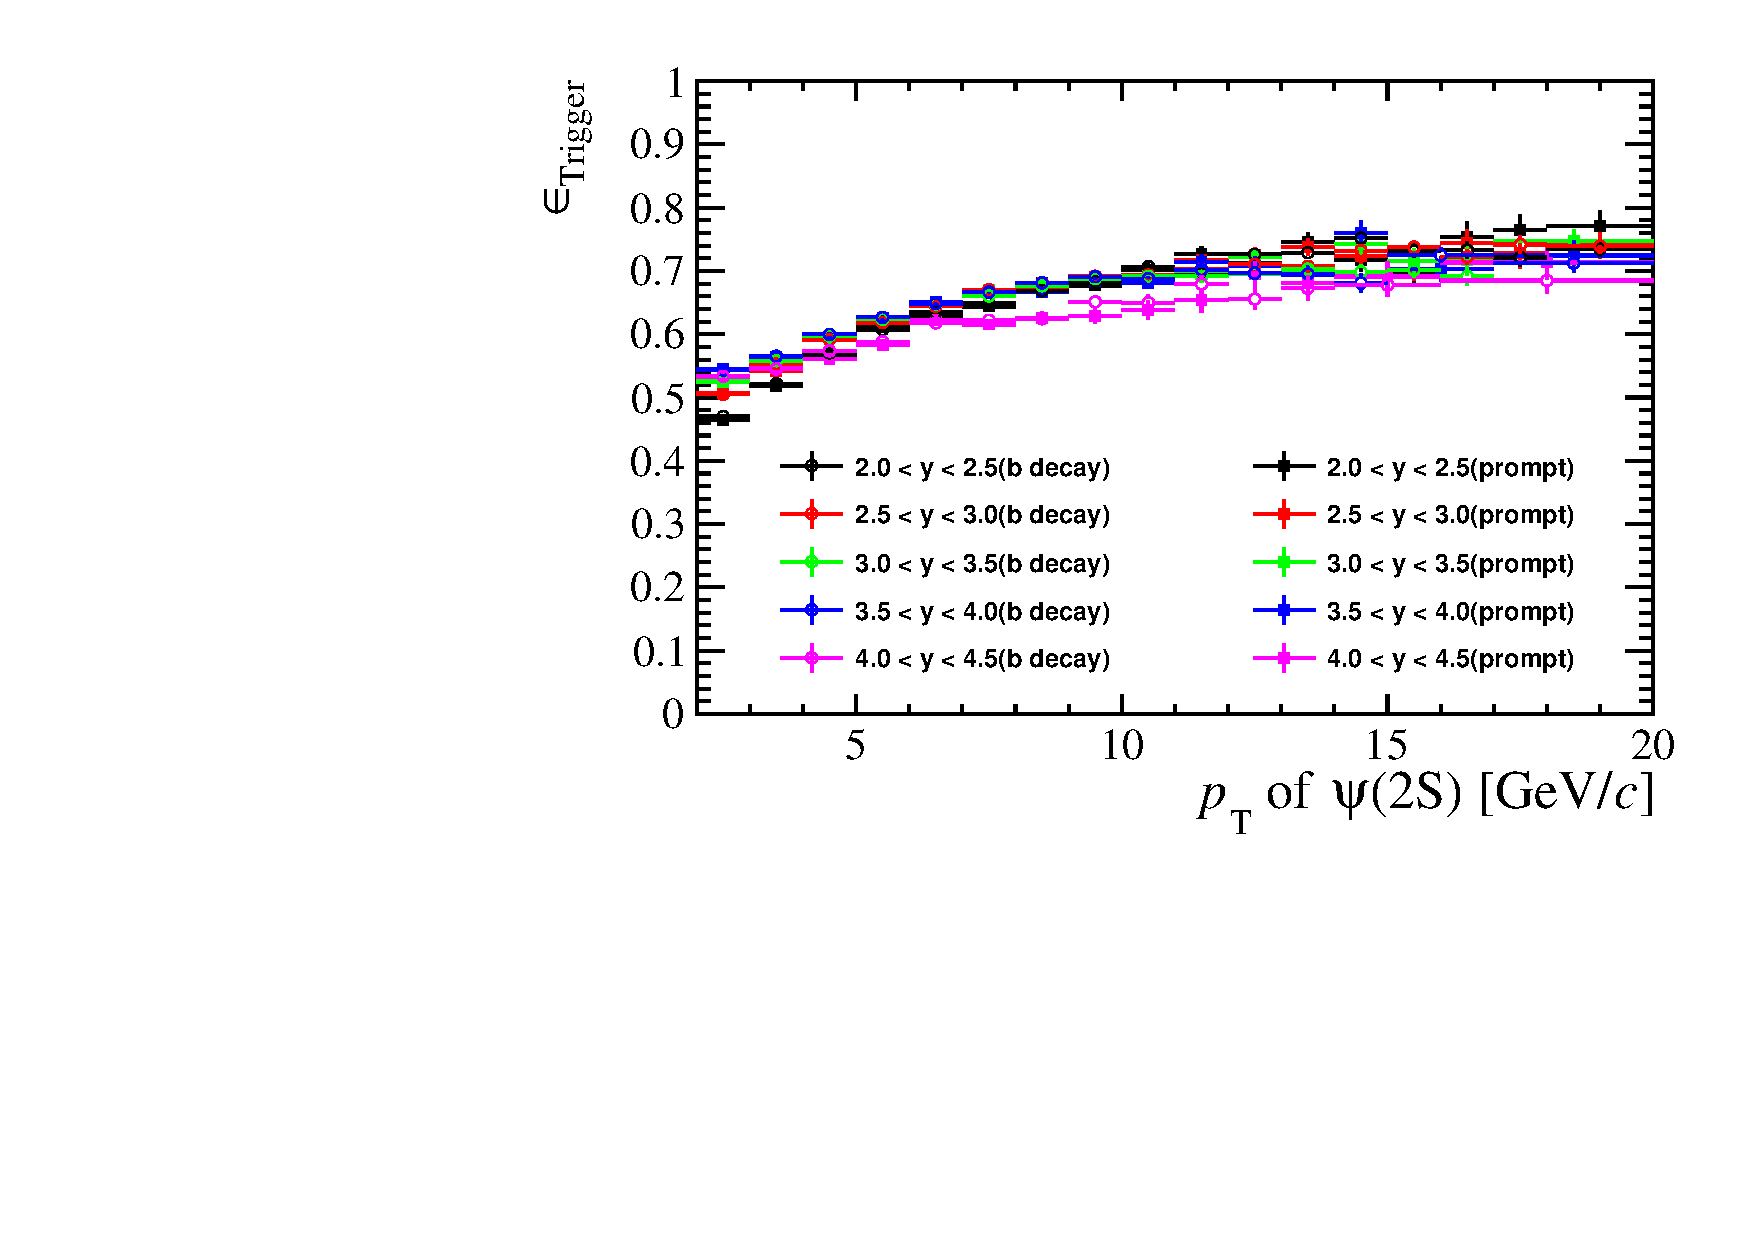
\includegraphics[width=0.9\textwidth]{chap3_eff_trigger_compare}
\caption{以$\pt$、$y$为函数的触发效率分布。}
\label{fig:EffTrigger}
\end{figure}

\subsection{总的效率}\label{sec:tot_eff}
$\pp$对撞直接产生的$\psitwos$介子和来自$b$强子衰变产生的$\psitwos$介子的总效率图如~\ref{fig:EffTot_compare}所示。
总效率的数值结果,我们总结在附录~\ref{sec:EffTables}的表~\ref{tab:efftot_prompt}和表~\ref{tab:efftot_bdecay}中。
为了方便比较,我们讲直接产生的$\psitwos$和来自于$b$强子衰变来的$\psitwos$的总效率做了个比值放在图~\ref{fig:EffTot_ratio}。
我们注意到二者效率基本是一致的。
%%%%%%%%%%%%%%%%%%%%%%%%%%%%%%%%%%%%%%%%%%%%%%%%%%%%%%%%%%%
\begin{figure}[!tbp]
\centering
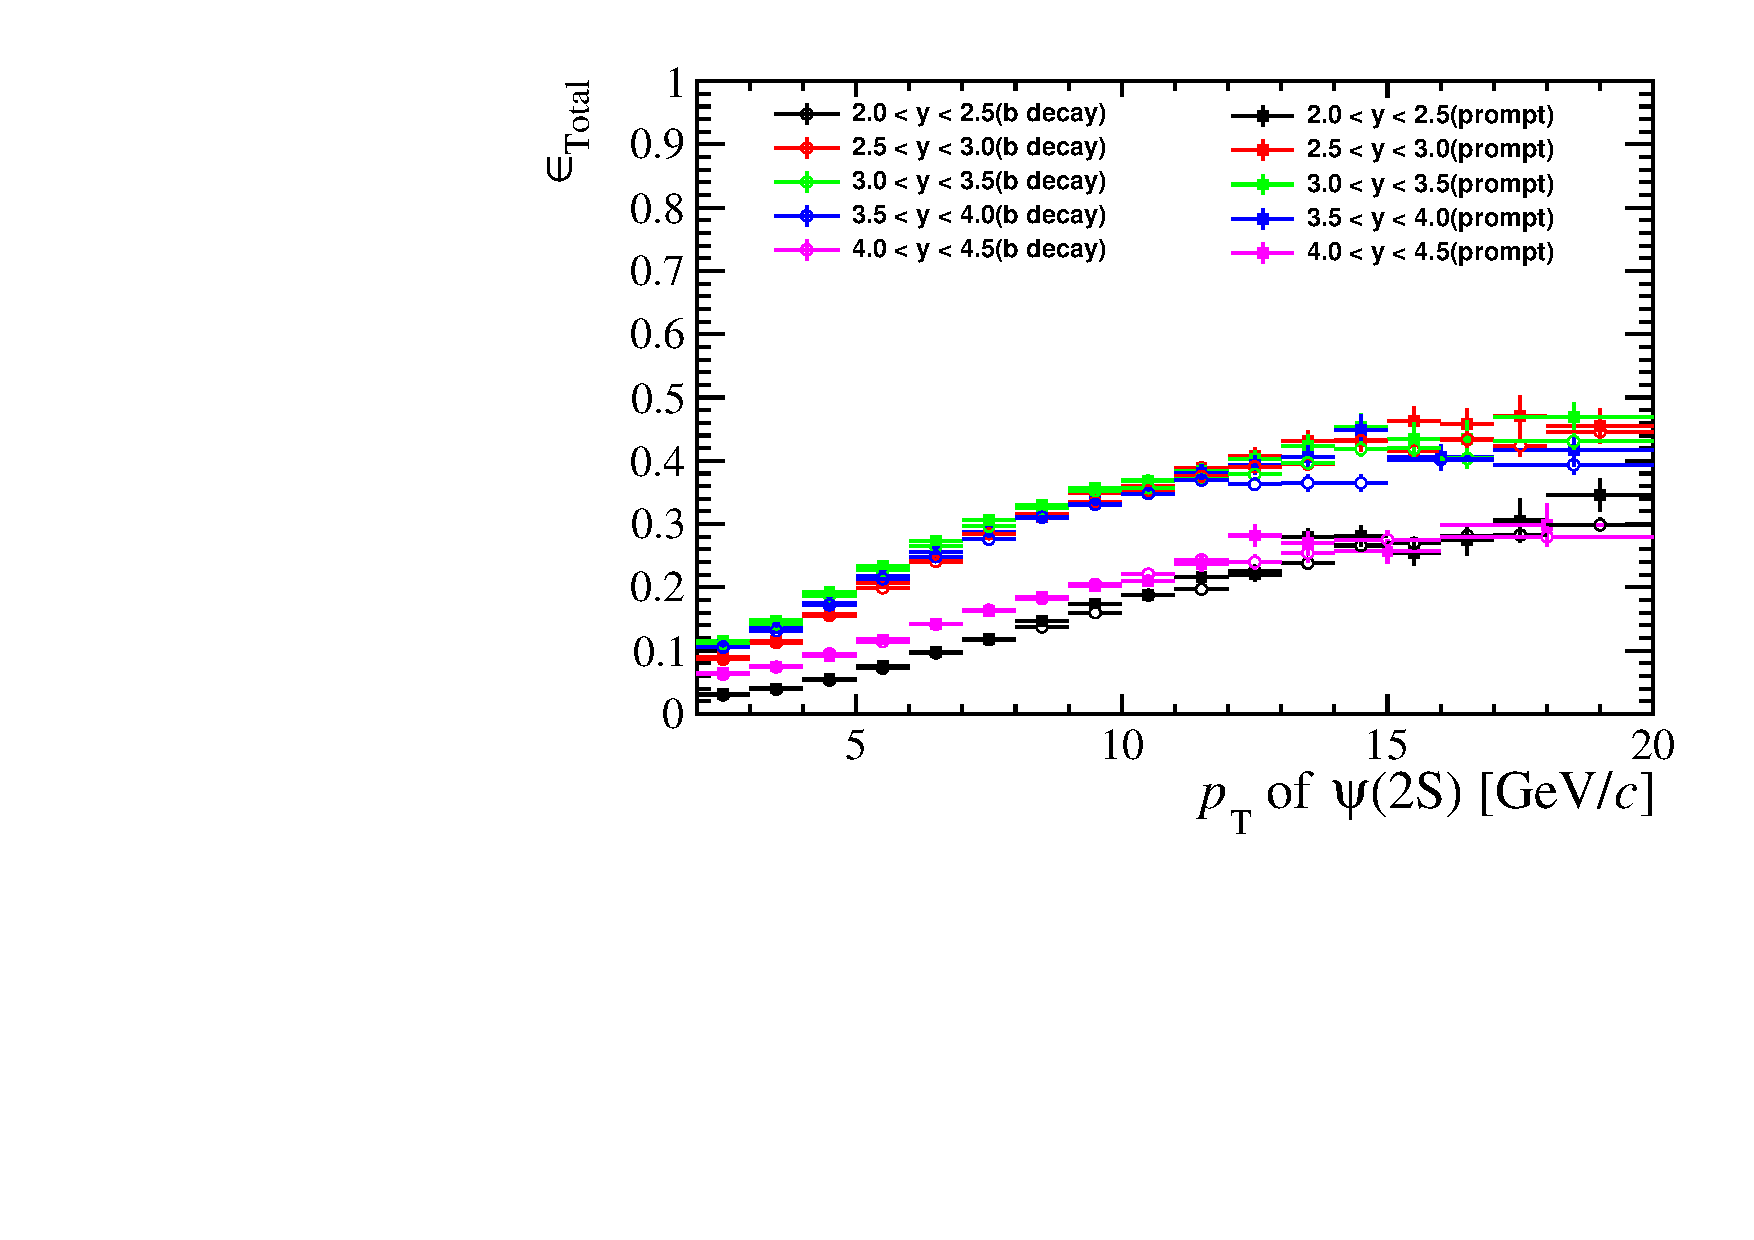
\includegraphics[width=0.9\textwidth]{chap3_eff_compare}
\caption{ 在不同的$\pt$ 和 $y$区间内,$\psitwos$的总效率分布。}
\label{fig:EffTot_compare}
\end{figure}

%%%%%%%%%%%%%%%%%%%%%%%%%%%%%%%%%%%%%%%%%%%%%%%%%%%%%%%%%%%
\begin{figure}[!tbp]
\centering
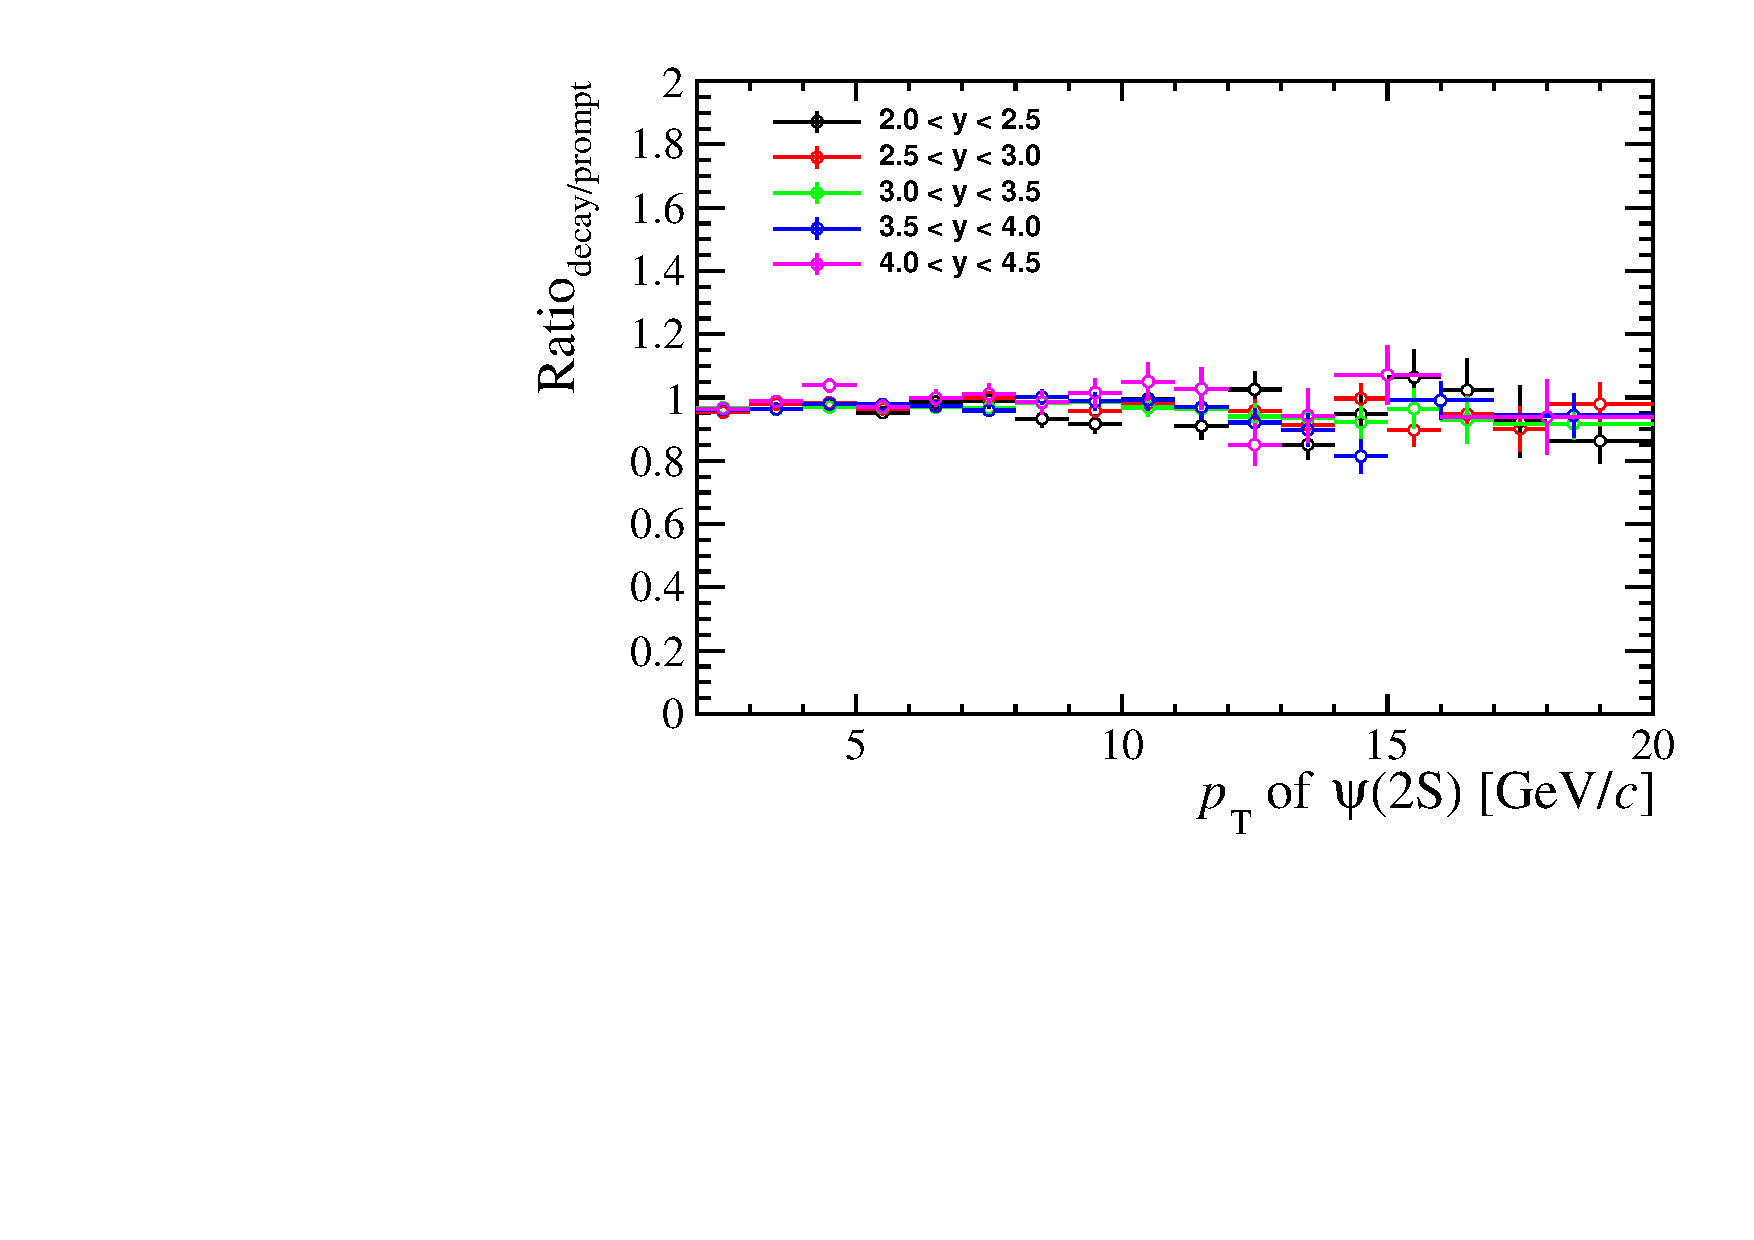
\includegraphics[width=0.9\textwidth]{chap3_eff_ratio_BP.pdf}
\caption{ 在不同的$\pt$ 和 $y$区间内,直接产生的$\psitwos$和来自于$b$强子衰变来的$\psitwos$的总效率比值。}
\label{fig:EffTot_ratio}
\end{figure}
%%%%%%%%%%%%%%%%%%%%%%%%%%%%%%%%%%%%%%%%%%%%%%%%%%%%%%%%%%%

